% Options for packages loaded elsewhere
\PassOptionsToPackage{unicode}{hyperref}
\PassOptionsToPackage{hyphens}{url}
%
\documentclass[
]{article}
\usepackage{lmodern}
\usepackage{amssymb,amsmath}
\usepackage{ifxetex,ifluatex}
\ifnum 0\ifxetex 1\fi\ifluatex 1\fi=0 % if pdftex
  \usepackage[T1]{fontenc}
  \usepackage[utf8]{inputenc}
  \usepackage{textcomp} % provide euro and other symbols
\else % if luatex or xetex
  \usepackage{unicode-math}
  \defaultfontfeatures{Scale=MatchLowercase}
  \defaultfontfeatures[\rmfamily]{Ligatures=TeX,Scale=1}
\fi
% Use upquote if available, for straight quotes in verbatim environments
\IfFileExists{upquote.sty}{\usepackage{upquote}}{}
\IfFileExists{microtype.sty}{% use microtype if available
  \usepackage[]{microtype}
  \UseMicrotypeSet[protrusion]{basicmath} % disable protrusion for tt fonts
}{}
\makeatletter
\@ifundefined{KOMAClassName}{% if non-KOMA class
  \IfFileExists{parskip.sty}{%
    \usepackage{parskip}
  }{% else
    \setlength{\parindent}{0pt}
    \setlength{\parskip}{6pt plus 2pt minus 1pt}}
}{% if KOMA class
  \KOMAoptions{parskip=half}}
\makeatother
\usepackage{xcolor}
\IfFileExists{xurl.sty}{\usepackage{xurl}}{} % add URL line breaks if available
\IfFileExists{bookmark.sty}{\usepackage{bookmark}}{\usepackage{hyperref}}
\hypersetup{
  pdftitle={Clase 5 - El paquete GGPlot2},
  hidelinks,
  pdfcreator={LaTeX via pandoc}}
\urlstyle{same} % disable monospaced font for URLs
\usepackage[margin=1in]{geometry}
\usepackage{color}
\usepackage{fancyvrb}
\newcommand{\VerbBar}{|}
\newcommand{\VERB}{\Verb[commandchars=\\\{\}]}
\DefineVerbatimEnvironment{Highlighting}{Verbatim}{commandchars=\\\{\}}
% Add ',fontsize=\small' for more characters per line
\usepackage{framed}
\definecolor{shadecolor}{RGB}{248,248,248}
\newenvironment{Shaded}{\begin{snugshade}}{\end{snugshade}}
\newcommand{\AlertTok}[1]{\textcolor[rgb]{0.94,0.16,0.16}{#1}}
\newcommand{\AnnotationTok}[1]{\textcolor[rgb]{0.56,0.35,0.01}{\textbf{\textit{#1}}}}
\newcommand{\AttributeTok}[1]{\textcolor[rgb]{0.77,0.63,0.00}{#1}}
\newcommand{\BaseNTok}[1]{\textcolor[rgb]{0.00,0.00,0.81}{#1}}
\newcommand{\BuiltInTok}[1]{#1}
\newcommand{\CharTok}[1]{\textcolor[rgb]{0.31,0.60,0.02}{#1}}
\newcommand{\CommentTok}[1]{\textcolor[rgb]{0.56,0.35,0.01}{\textit{#1}}}
\newcommand{\CommentVarTok}[1]{\textcolor[rgb]{0.56,0.35,0.01}{\textbf{\textit{#1}}}}
\newcommand{\ConstantTok}[1]{\textcolor[rgb]{0.00,0.00,0.00}{#1}}
\newcommand{\ControlFlowTok}[1]{\textcolor[rgb]{0.13,0.29,0.53}{\textbf{#1}}}
\newcommand{\DataTypeTok}[1]{\textcolor[rgb]{0.13,0.29,0.53}{#1}}
\newcommand{\DecValTok}[1]{\textcolor[rgb]{0.00,0.00,0.81}{#1}}
\newcommand{\DocumentationTok}[1]{\textcolor[rgb]{0.56,0.35,0.01}{\textbf{\textit{#1}}}}
\newcommand{\ErrorTok}[1]{\textcolor[rgb]{0.64,0.00,0.00}{\textbf{#1}}}
\newcommand{\ExtensionTok}[1]{#1}
\newcommand{\FloatTok}[1]{\textcolor[rgb]{0.00,0.00,0.81}{#1}}
\newcommand{\FunctionTok}[1]{\textcolor[rgb]{0.00,0.00,0.00}{#1}}
\newcommand{\ImportTok}[1]{#1}
\newcommand{\InformationTok}[1]{\textcolor[rgb]{0.56,0.35,0.01}{\textbf{\textit{#1}}}}
\newcommand{\KeywordTok}[1]{\textcolor[rgb]{0.13,0.29,0.53}{\textbf{#1}}}
\newcommand{\NormalTok}[1]{#1}
\newcommand{\OperatorTok}[1]{\textcolor[rgb]{0.81,0.36,0.00}{\textbf{#1}}}
\newcommand{\OtherTok}[1]{\textcolor[rgb]{0.56,0.35,0.01}{#1}}
\newcommand{\PreprocessorTok}[1]{\textcolor[rgb]{0.56,0.35,0.01}{\textit{#1}}}
\newcommand{\RegionMarkerTok}[1]{#1}
\newcommand{\SpecialCharTok}[1]{\textcolor[rgb]{0.00,0.00,0.00}{#1}}
\newcommand{\SpecialStringTok}[1]{\textcolor[rgb]{0.31,0.60,0.02}{#1}}
\newcommand{\StringTok}[1]{\textcolor[rgb]{0.31,0.60,0.02}{#1}}
\newcommand{\VariableTok}[1]{\textcolor[rgb]{0.00,0.00,0.00}{#1}}
\newcommand{\VerbatimStringTok}[1]{\textcolor[rgb]{0.31,0.60,0.02}{#1}}
\newcommand{\WarningTok}[1]{\textcolor[rgb]{0.56,0.35,0.01}{\textbf{\textit{#1}}}}
\usepackage{graphicx}
\makeatletter
\def\maxwidth{\ifdim\Gin@nat@width>\linewidth\linewidth\else\Gin@nat@width\fi}
\def\maxheight{\ifdim\Gin@nat@height>\textheight\textheight\else\Gin@nat@height\fi}
\makeatother
% Scale images if necessary, so that they will not overflow the page
% margins by default, and it is still possible to overwrite the defaults
% using explicit options in \includegraphics[width, height, ...]{}
\setkeys{Gin}{width=\maxwidth,height=\maxheight,keepaspectratio}
% Set default figure placement to htbp
\makeatletter
\def\fps@figure{htbp}
\makeatother
\setlength{\emergencystretch}{3em} % prevent overfull lines
\providecommand{\tightlist}{%
  \setlength{\itemsep}{0pt}\setlength{\parskip}{0pt}}
\setcounter{secnumdepth}{-\maxdimen} % remove section numbering

\title{Clase 5 - El paquete GGPlot2}
\author{}
\date{\vspace{-2.5em}}

\begin{document}
\maketitle

Ggplot 2 es el paquete más avanzado en R. Utiliza la gramática de los
gráficos y permite crear visualizaciones tan personalizadas como cuanto
uno quiera. Pertenece al paquete tidiverse.

\begin{itemize}
\tightlist
\item
  ReadR - Importa datos en diversos formatos, siendo el mejor ejemplo
  \texttt{read\_csv()}
\item
  Tibble - Crea una estructura de datos similar a la data frame que
  facilita la manipulacion de datos
\item
  Permite filtrar resumir y manipular datos
\item
  tidyr - Organiza datos en forma tidy
\end{itemize}

Lo primero que debemos hacer es cargar la library, ya sea mediante
invocando todo el \texttt{tidyverse} (recomendado) o unicamente
\texttt{ggplot2}

\begin{verbatim}
## -- Attaching packages ------------------------------------------------------------------------------------------------------------- tidyverse 1.3.0 --
\end{verbatim}

\begin{verbatim}
## v ggplot2 3.3.2     v purrr   0.3.4
## v tibble  3.0.2     v dplyr   1.0.0
## v tidyr   1.1.0     v stringr 1.4.0
## v readr   1.3.1     v forcats 0.5.0
\end{verbatim}

\begin{verbatim}
## -- Conflicts ---------------------------------------------------------------------------------------------------------------- tidyverse_conflicts() --
## x dplyr::filter() masks stats::filter()
## x dplyr::lag()    masks stats::lag()
\end{verbatim}

A continuacion vamos a realizar los graficos

\hypertarget{gramatica-de-graficos}{%
\subsection{Gramatica de graficos}\label{gramatica-de-graficos}}

La gramatica de graficos es el andamiaje que permite crear y
personalizar los graficos desde cero, proveyendo una fuente de datos.
Los elementos más básicos de esta gramática son:

\begin{itemize}
\tightlist
\item
  La fuente de datos que uno va a utilizar (\texttt{data})
\item
  La forma que va a tomar los datos en la visualizacion, o su geometria
  (\texttt{geom}), por ejemplo puntos, líneas, barras.
\item
  Las propiedades esteticas (aesthetics) de las geometrias \texttt{aes}
  por ejemplo qué datos van en los ejes, representar un color para una
  variable, o el diametro de un punto para otra.
\end{itemize}

Otros elementos de la gramática son \texttt{scales}, \#\#\#, etc.

\hypertarget{iniciando-en-ggplot2}{%
\subsection{Iniciando en ggplot2}\label{iniciando-en-ggplot2}}

La primera visualizacion que vamos a realizar esta basada en la base de
datos \texttt{iris} que contiene las medidas de tres especies del genero
\emph{Iris}: \emph{setosa, virginica y versicolor}.

\begin{figure}
\centering
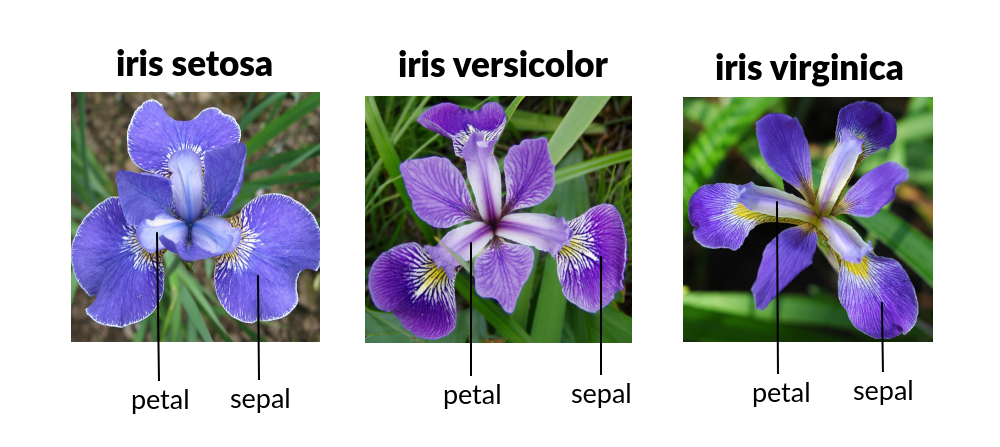
\includegraphics{iris.png}
\caption{\textbf{Flores de \emph{Iris}}}
\end{figure}

Una vez cargada la library, podemos ejecutar por primera vez el comando
\texttt{ggplot} OJO SIN EL 2 AL FINAL! (si, es confuso para la mierda,
pero bueno es lo que hay). Al ejecutarlo sin parametros, observamos que
nos muestra un grafico totalmente en blanco.

\begin{Shaded}
\begin{Highlighting}[]
\KeywordTok{ggplot}\NormalTok{()}
\end{Highlighting}
\end{Shaded}

\includegraphics{Clase-5_files/figure-latex/unnamed-chunk-2-1.pdf}

Si ahora especificamos la fuente de los datos en el parametro
\texttt{data\ =}:

\begin{Shaded}
\begin{Highlighting}[]
\KeywordTok{ggplot}\NormalTok{(}\DataTypeTok{data =}\NormalTok{ iris)}
\end{Highlighting}
\end{Shaded}

\includegraphics{Clase-5_files/figure-latex/unnamed-chunk-3-1.pdf}

Nuevamente no tenemos ninguna salida significativa. Creemos un grafico
de puntos con los datos que tenemos, simplemente agregando mas
informacion (naturalmetne, utilizando el signo ``+'') sobre la geometria
que vamos a trabajar. En ggplot, todas las geometrias funcionan con el
prefijo \texttt{geom\_} asi que resulta fácil encontrarlas cuando las
necesitemos. Para orientar a la funcion qué es lo que vamos a mapear en
sus coordenadas, utilizaremos el parámetro \texttt{mapping\ =}, seguido
de la funcion que define las propiedades esteticas del grafico
\texttt{aes()}.

\begin{Shaded}
\begin{Highlighting}[]
\KeywordTok{ggplot}\NormalTok{(}\DataTypeTok{data =}\NormalTok{ iris) }\OperatorTok{+}
\StringTok{  }\KeywordTok{geom\_point}\NormalTok{(}\DataTypeTok{mapping =} \KeywordTok{aes}\NormalTok{(}\DataTypeTok{x =}\NormalTok{ Species, }\DataTypeTok{y =}\NormalTok{ Petal.Length))}
\end{Highlighting}
\end{Shaded}

\includegraphics{Clase-5_files/figure-latex/unnamed-chunk-4-1.pdf}

Ahora continuamos con otra de las bases del paquete ``nativo'' (que ya
viene preinstalado en R) \texttt{trees}. Veamos que contiene acudiendo a
la ayuda.

\begin{Shaded}
\begin{Highlighting}[]
\KeywordTok{help}\NormalTok{(}\StringTok{"trees"}\NormalTok{)}
\end{Highlighting}
\end{Shaded}

\begin{verbatim}
## starting httpd help server ... done
\end{verbatim}

Sabremos entonces que la database tiene 3 variables: diametro, altura y
volumen del cerecero negro.

Ahora vamos a continuar haciendo un scatterplot, utilizando la geometria
point, siguiendo los mismos pasos que el caso anterior.

\begin{Shaded}
\begin{Highlighting}[]
\KeywordTok{ggplot}\NormalTok{(}\DataTypeTok{data =}\NormalTok{ trees) }\OperatorTok{+}\StringTok{ }
\StringTok{  }\KeywordTok{geom\_point}\NormalTok{(}\DataTypeTok{mapping =} \KeywordTok{aes}\NormalTok{(}\DataTypeTok{x =}\NormalTok{ Girth, }\DataTypeTok{y =}\NormalTok{ Volume))}
\end{Highlighting}
\end{Shaded}

\includegraphics{Clase-5_files/figure-latex/unnamed-chunk-6-1.pdf}

\textbf{Cuidado que esta representacion o tiene al 0 como origen!}
Despues veremos como resolver esta cuestión.

Podemos maximizar la información de este grafico, mapeando la tercer
variable, \texttt{Volume} en pies cubicos, a otra de las estéticas de
los puntos, el parametro \texttt{color\ =}:

\begin{Shaded}
\begin{Highlighting}[]
\KeywordTok{ggplot}\NormalTok{(}\DataTypeTok{data =}\NormalTok{ trees) }\OperatorTok{+}\StringTok{ }
\StringTok{  }\KeywordTok{geom\_point}\NormalTok{(}\DataTypeTok{mapping =} \KeywordTok{aes}\NormalTok{(}\DataTypeTok{x =}\NormalTok{ Girth, }\DataTypeTok{y =}\NormalTok{ Volume, }\DataTypeTok{color =}\NormalTok{ Volume))}
\end{Highlighting}
\end{Shaded}

\includegraphics{Clase-5_files/figure-latex/unnamed-chunk-7-1.pdf}

\end{document}
